\chapter{Kekorakenteet}

Keko on nimitys puurakenteelle, jossa jokainen solmu toteuttaa kekoehdon.
Minimikeossa ehtona on, että jokaisen solmun arvo on suurempi tai yhtä suuri
kuin solmun vanhemman arvo.
Maksimikeossa taas jokaisen solmun arvo on pienempi
tai yhtä suuri kuin solmun vanhemman arvo.

Tässä luvussa tutustumme binäärikekoon,
joka pitää yllä alkioiden joukkoa ja tarjoaa seuraavat tehokkaat operaatiot:

\begin{itemize}
\item lisää alkio joukkoon
\item etsi joukon pienin/suurin alkio
\item poista joukon pienin/suurin alkio
\end{itemize}

Minimikeossa kaksi jälkimmäistä operaatiota etsivät tai poistavat pienimmän alkion.
Maksimikeossa taas operaatiot etsivät tai poistavat suurimman alkion.

Huomaa, että voimme toteuttaa yllä olevat operaatiot ja enemmänkin
myös binäärihakupuun avulla.
Keossa voimme vain etsiä ja poistaa joukon pienimmän/suurimman alkion,
kun taas binäärihakupuussa voimme etsiä ja poistaa mitä tahansa alkioita.
Keon etuna on kuitenkin, että sen rakenne on binäärihakupuuta
yksinkertaisempi, minkä ansiosta sen tarjoamat operaatiot toimivat
nopeammin kuin vastaavat binäärihakupuun operaatiot.

\section{Binäärikeko}

Oletamme tästä lähtien, että haluamme toteuttaa binäärikeon,
joka toimii minimikekona, eli jokaisen solmun arvo on suurempi
tai yhtä suuri kuin solmun vanhemman arvo.
Binäärikeossa puuta ''täytetään'' ylhäältä alas ja vasemmalta oikealle,
eli puun ensimmäiset kerrokset ovat mahdollisimman täynnä solmuja
ja viimeisessä kerroksessa solmut ovat mahdollisimman vasemmalla.

Kuvassa \ref{fig:minkek} on esimerkkinä joukkoa $\{1,2,3,3,5,8\}$
vastaava minimikeko.
Tässä tapaukessa puun kaksi ensimmäistä kerrosta ovat täynnä,
ja kolmannessa kerroksessa kolme ensimmäistä kohtaa on käytetty.
Huomaa, että sama alkio voi esiintyä keossa monta kertaa,
kuten tässä joukossa esiintyy kaksi kertaa alkio 3.

\begin{figure}
\center
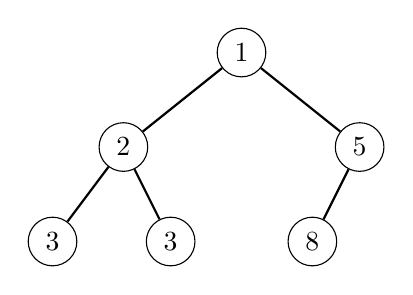
\begin{tikzpicture}[scale=0.6]
\node[draw, circle] (1) at (0,0) {$1$};
\node[draw, circle] (2) at (-2.5,-2) {$2$};
\node[draw, circle] (3) at (2.5,-2) {$5$};
\node[draw, circle] (4) at (-4,-4) {$3$};
\node[draw, circle] (5) at (-1.5,-4) {$3$};
\node[draw, circle] (6) at (1.5,-4) {$8$};
\path[draw,thick,-] (1) -- (2);
\path[draw,thick,-] (1) -- (3);
\path[draw,thick,-] (2) -- (4);
\path[draw,thick,-] (2) -- (5);
\path[draw,thick,-] (3) -- (6);
\end{tikzpicture}
\caption{Minimikeko, joka vastaa joukkoa $\{1,2,3,3,5,8\}$.}
\label{fig:minkek}
\end{figure}

\subsection{Operaatiot}

Meidän on helppoa etsiä minimikeon pienin alkio $O(1)$-ajassa,
koska se on aina keon juuressa.
Seuraavaksi näemme, kuinka voimme toteuttaa alkion lisäämisen
sekä pienimmän alkion poistamisen $O(\log n)$-ajassa.

\subsubsection{Alkion lisääminen}

Kun lisäämme uuden alkion kekoon, lisäämme sen ensin seuraavaan
vapaana olevaan paikkaan. Jos alimmalla kerroksella on tilaa,
lisäämme sen sinne mahdollisimman vasemmalle,
ja muuten aloitamme uuden kerroksen, jossa on vain uusi solmu.

Alkion lisäämisen jälkeen meidän täytyy varmistaa,
että kekoehto säilyy edelleen voimassa.
Tämä tapahtuu siirtämällä alkiota ylöspäin keossa
niin kauan kuin se on vanhempaansa pienempi.
Koska täytämme kekoa tasaisesti, sen korkeus on $O(\log n)$
ja operaatio toimii $O(\log n)$-ajassa.

\begin{figure}
\center
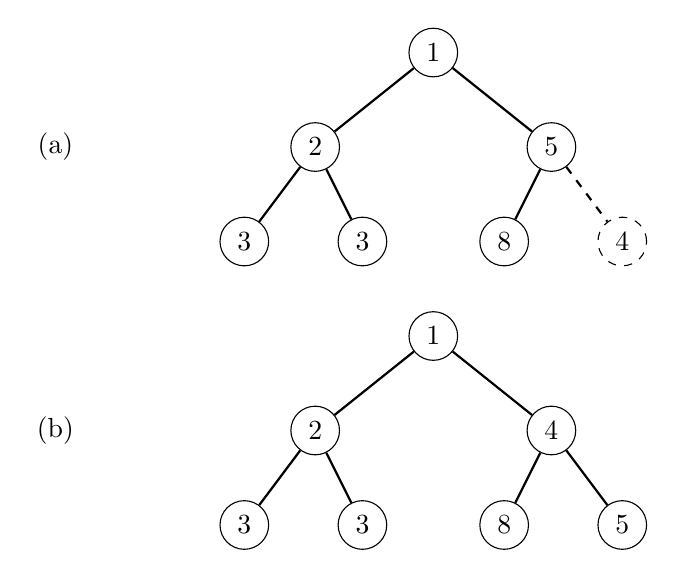
\begin{tikzpicture}[scale=0.6]
\begin{scope}
\node at (-8,-2) {(a)};
\node[draw, circle] (1) at (0,0) {$1$};
\node[draw, circle] (2) at (-2.5,-2) {$2$};
\node[draw, circle] (3) at (2.5,-2) {$5$};
\node[draw, circle] (4) at (-4,-4) {$3$};
\node[draw, circle] (5) at (-1.5,-4) {$3$};
\node[draw, circle] (6) at (1.5,-4) {$8$};
\node[draw, circle, dashed] (7) at (4,-4) {$4$};
\path[draw,thick,-] (1) -- (2);
\path[draw,thick,-] (1) -- (3);
\path[draw,thick,-] (2) -- (4);
\path[draw,thick,-] (2) -- (5);
\path[draw,thick,-] (3) -- (6);
\path[draw,thick,-,dashed] (3) -- (7);
\end{scope}
\begin{scope}[yshift=-6cm]
\node at (-8,-2) {(b)};
\node[draw, circle] (1) at (0,0) {$1$};
\node[draw, circle] (2) at (-2.5,-2) {$2$};
\node[draw, circle] (3) at (2.5,-2) {$4$};
\node[draw, circle] (4) at (-4,-4) {$3$};
\node[draw, circle] (5) at (-1.5,-4) {$3$};
\node[draw, circle] (6) at (1.5,-4) {$8$};
\node[draw, circle] (7) at (4,-4) {$5$};
\path[draw,thick,-] (1) -- (2);
\path[draw,thick,-] (1) -- (3);
\path[draw,thick,-] (2) -- (4);
\path[draw,thick,-] (2) -- (5);
\path[draw,thick,-] (3) -- (6);
\path[draw,thick,-] (3) -- (7);
\end{scope}
\end{tikzpicture}
\caption{Alkion 4 lisääminen kekoon. (a) Lisäämme alkion ensimmäiseen
vapaana olevaan paikkaan. (b) Koska alkio on vanhempaansa pienempi,
vaihdamme alkiot keskenään.}
\label{fig:keklis}
\end{figure}

Kuva \ref{fig:keklis} näyttää esimerkin alkion lisäämisestä kekoon.
Lisäämme ensin alkion 4 keon ensimmäiseen vapaana olevaan paikkaan.
Koska uuden solmun arvo on sen vanhemman arvoa pienempi,
vaihdamme nämä arvot keskenään. Tämän jälkeen kekoehto on voimassa.

\subsubsection{Pienimmän alkion poistaminen}

Kun haluamme poistaa keon pienimmän alkion, vaihdamme ensin keskenään
juuressa olevan pienimmän arvon sekä keon viimeisessä käytössä olevassa
paikassa olevan arvon. Tämän jälkeen poistamme keon viimeisen solmun,
jolloin pienin arvo katoaa keosta.

Tämän jälkeen meidän täytyy jälleen huolehtia siitä, että kekoehto pätee.
Tämä tapahtuu laskettamalla juuressa olevaa arvoa alaspäin keossa,
kunnes kekoehto pätee. Valitsemme aina kahdesta mahdollisesta suunnasta sen,
jossa on pienempi alkio.
Koska alkio laskeutuu enintään $O(\log n)$ askelta,
tämäkin operaatio toimii ajassa $O(\log n)$.

\begin{figure}
\center
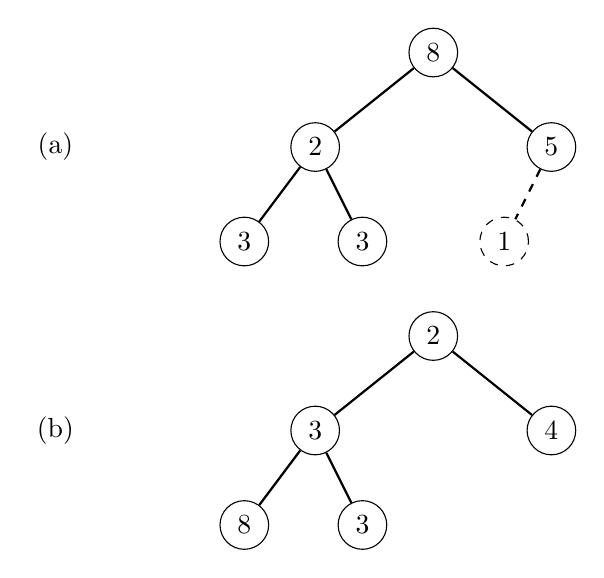
\begin{tikzpicture}[scale=0.6]
\begin{scope}
\node at (-8,-2) {(a)};
\node[draw, circle] (1) at (0,0) {$8$};
\node[draw, circle] (2) at (-2.5,-2) {$2$};
\node[draw, circle] (3) at (2.5,-2) {$5$};
\node[draw, circle] (4) at (-4,-4) {$3$};
\node[draw, circle] (5) at (-1.5,-4) {$3$};
\node[draw, circle, dashed] (6) at (1.5,-4) {$1$};
\path[draw,thick,-] (1) -- (2);
\path[draw,thick,-] (1) -- (3);
\path[draw,thick,-] (2) -- (4);
\path[draw,thick,-] (2) -- (5);
\path[draw,thick,-,dashed] (3) -- (6);
\end{scope}
\begin{scope}[yshift=-6cm]
\node at (-8,-2) {(b)};
\node[draw, circle] (1) at (0,0) {$2$};
\node[draw, circle] (2) at (-2.5,-2) {$3$};
\node[draw, circle] (3) at (2.5,-2) {$4$};
\node[draw, circle] (4) at (-4,-4) {$8$};
\node[draw, circle] (5) at (-1.5,-4) {$3$};
\path[draw,thick,-] (1) -- (2);
\path[draw,thick,-] (1) -- (3);
\path[draw,thick,-] (2) -- (4);
\path[draw,thick,-] (2) -- (5);
\end{scope}
\end{tikzpicture}
\caption{Pienimmän alkion poistaminen keosta. (a) Vaihdamme keskenään
pienimmän alkion ja viimeisen alkion. (b) Alkio 8 laskeutuu keon
huipulta takaisin sen pohjalle.}
\label{fig:kekpoi}
\end{figure}

Kuva \ref{fig:kekpoi} näyttää esimerkin alkion poistamisesta keosta.
Aluksi vaihdamme keskenään keon pienimmän alkion $1$
ja viimeisenä keossa olevan alkion $8$.
Tämän jälkeen lasketamme alkiota $8$ juuresta alaspäin,
kunnes kekoehto on voimassa.
Tässä tapauksessa alkio laskeutuu keon pohjalle asti.

\subsection{Toteutus taulukkona}

Kätevä tapa toteuttaa keko on tallentaa sen solmujen
sisältö taulukkoon järjestyksessä ylhäältä alas ja vasemmalta oikealle.
Jotta voimme toteuttaa mukavasti keon operaatiot,
käytämme 1-indeksoitua taulukkoa.
Kuva \ref{fig:kektau} näyttää esimerkin keon tallentamisesta taulukkoon.

\begin{figure}
\center
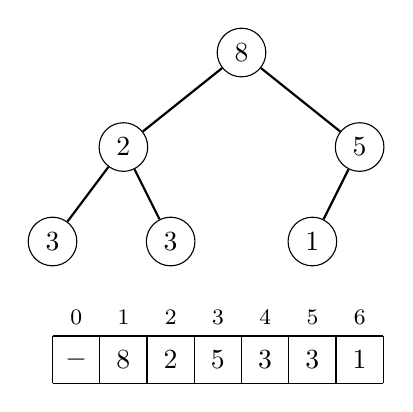
\begin{tikzpicture}[scale=0.6]
\begin{scope}
\node[draw, circle] (1) at (0,0) {$8$};
\node[draw, circle] (2) at (-2.5,-2) {$2$};
\node[draw, circle] (3) at (2.5,-2) {$5$};
\node[draw, circle] (4) at (-4,-4) {$3$};
\node[draw, circle] (5) at (-1.5,-4) {$3$};
\node[draw, circle] (6) at (1.5,-4) {$1$};
\path[draw,thick,-] (1) -- (2);
\path[draw,thick,-] (1) -- (3);
\path[draw,thick,-] (2) -- (4);
\path[draw,thick,-] (2) -- (5);
\path[draw,thick,-] (3) -- (6);
\end{scope}
\begin{scope}[yshift=-7cm,xshift=-4cm]
\draw (0,0) grid (7,1);
\node at (0.5,0.5) {$-$};
\node at (1.5,0.5) {$8$};
\node at (2.5,0.5) {$2$};
\node at (3.5,0.5) {$5$};
\node at (4.5,0.5) {$3$};
\node at (5.5,0.5) {$3$};
\node at (6.5,0.5) {$1$};
\footnotesize
\node at (0.5,1.4) {$0$};
\node at (1.5,1.4) {$1$};
\node at (2.5,1.4) {$2$};
\node at (3.5,1.4) {$3$};
\node at (4.5,1.4) {$4$};
\node at (5.5,1.4) {$5$};
\node at (6.5,1.4) {$6$};
\end{scope}
\end{tikzpicture}
\caption{Keko ja sen taulukkoesitys.}
\label{fig:kektau}
\end{figure}

Kun meillä on tiedossa solmun kohta taulukossa,
voimme helposti selvittää sen lasten ja vanhemman kohdat.
Kohdassa $k$ olevan solmun vasen lapsi on kohdassa $2k$
ja oikea lapsi on kohdassa $2k+1$.
Lisäksi solmun vanhempi on kohdassa $\lfloor k/2 \rfloor$.
Tämän ansiosta voimme toteuttaa keon operaatiot niin,
että niiden vakiokertoimet ovat pienet.

\subsection{Tehokas luonti}

Suoraviivainen tapa luoda $n$ alkiota sisältävä keko
on lisätä jokainen alkio erikseen kekoon $O(\log n)$-ajassa.
Tällä tavalla saamme rakennettua keon $O(n \log n)$-ajassa.
Osoittautuu kuitenkin, että keon luominen taulukon pohjalta
on mahdollista myös $O(n)$-ajassa.

Ideana on käydä läpi keon solmut lopusta alkuun ja
jokaisen solmun kohdalla varmistaa,
että siitä solmusta alkava alipuu toteuttaa kekoehdon
laskettamalla solmun juuressa olevaa arvoa alaspäin.
Kun olemme lopulta käsitelleet kaikki solmut juureen asti,
koko taulukko toteuttaa kekoehdon.

Miksi sitten tämä vie aikaa vain $O(n)$?
Oletetaan, että keossa on $h$ kerrosta ja kaikki
kerrokset ovat täynnä solmuja, eli siinä on $n=2^h-1$ solmua.
Laskemme jokaiseen solmuun, montako kertaa enintään jokin
arvo laskeutuu alaspäin tästä solmusta. Tästä saamme:

\begin{itemize}
\item Kerroksesta 1 kerrokseen 2 laskeutuu enintään 1 arvo.
\item Kerroksesta 2 kerrokseen 3 laskeutuu enintään $1+2$ arvoa.
\item Kerroksesta 3 kerrokseen 4 laskeutuu enintään $1+2+4$ arvoa.
\item Jne.
\end{itemize}

Yleisemmin kerroksesta $k$ kerrokseen $k+1$ laskeutuu
enintään $1+2+\dots+2^{k-1} = 2^k-1$ arvoa.
Koska kerroksia on $h$ ja viimeisestä kerroksesta ei voi laskeutua alaspäin,
kokonaistyömäärä on enintään
\[(2^1-1)+(2^2-1)+\dots+(2^{h-1}-1)=2^h-h \le n,\]
joten aikaa kuluu vain $O(n)$.

\section{Javan toteutus}

\subsection{\texttt{PriorityQueue}}

\subsection{Kekotyypin valinta}

\section{Tehokkuusvertailu}

\section{Kekojärjestäminen}
